
 \documentclass[xcolor=table]{beamer}
\mode<presentation> {

% The Beamer class comes with a number of default slide themes
% which change the colors and layouts of slides. Below this is a list
% of all the themes, uncomment each in turn to see what they look like.

% \usetheme{default}
%\usetheme{AnnArbor}
%\usetheme{Antibes}
%\usetheme{Bergen}
%\usetheme{Berkeley}����JFIF����C
%\usetheme{Berlin}
%\usetheme{Boadilla}
%\usetheme{CambridgeUS}
%\usetheme{Copenhagen}
%\usetheme{Darmstadt}
%\usetheme{Dresden}
\usetheme{Frankfurt}
% \usetheme{Goettingen}
% \usetheme{Hannover}
%\usetheme{Ilmenau}
% \usetheme{JuanLesPins}
% \usetheme{Luebeck}
% \usetheme{Madrid}
% \usetheme{Malmoe}
% \usetheme{Marburg}
%\usetheme{Montpellier}
% \usetheme{PaloAlto}
\usetheme{Pittsburgh}
%\usetheme{Rochester}
%\usetheme{Singapore}
%\usetheme{Szeged}
% \usetheme{Warsaw}

% As well as themes, the Beamer class has a number of color themes
% for any slide theme. Uncomment each of these in turn to see how it
% changes the colors of your current slide theme.

% \usecolortheme{albatross}
%\usecolortheme{beaver}
%\usecolortheme{beetle}
% \usecolortheme{crane}
% \usecolortheme{dolphin}
 \usecolortheme{dove}
% \usecolortheme{fly}
% \usecolortheme{lily}
% \usecolortheme{orchid}
% \usecolortheme{rose}
% \usecolortheme{seagull}
% \usecolortheme{seahorse}
% \usecolortheme{whale}
% \usecolortheme{wolverine}
% \usecolortheme{dracula}

%\setbeamertemplate{footline} % To remove the footer line in all slides uncomment this line
\setbeamertemplate{footline}[page number] % To replace the footer line in all slides with a simple slide count uncomment this line

%\setbeamertemplate{navigation symbols}{} % To remove the navigation symbols from the bottom of all slides uncomment this line
}

% \usepackage[demo]{graphicx}

\usepackage[utf8]{inputenc}
\usepackage{neuralnetwork}
\usepackage{adjustbox}

\usepackage[para,online,flushleft]{threeparttable}
\usepackage{enumitem}
\usepackage{pifont}
\usepackage[normalem]{ulem}
\usepackage{listings}
\usepackage{xcolor}
\usepackage{minted}
\usepackage{textpos} 
\usepackage{hyperref}
\setbeamertemplate{caption}[numbered]

\defbeamertemplate{description item}{align left}{\insertdescriptionitem\hfill}
\beamertemplatenavigationsymbolsempty
\setbeamertemplate{description item}[align left]
%\usepackage{subcaption}
%----------------------------------------------------------------------------------------
%	TITLE PAGE
%----------------------------------------------------------------------------------------
\title[AI altering image detection]{Methods of detection of machine learing altered images }% The short title appears at the bottom of every slide, the full title is only on the title page

\author{Patryk Lisik } % Your name
\institute[] % Your institution as it will appear on the bottom of every slide, may be shorthand to save space
{
 Uniwersytet Łódzki \\ % Your institution for the title page
}

\date{2023/24}

%\addtobeamertemplate{frametitle}{}{%
%    \begin{textblock*}{100mm}(\textwidth,-1cm)
%        
\includegraphics[height=1cm,width=1cm]{falied-image-restoration.jpg}
%    \end{textblock*}
%
\begin{document}


\begin{frame}
\titlepage


% Print the title page as the first slide
\end{frame}

%----------------------------------------------------------------------------------
\section{Why this topic?}

\begin{frame}{Relevant}
    \begin{figure}
        \centering
        
\includegraphics[width=0.5\textwidth]{img/pope_balenciaga.jpg}
        \caption{Image known as  "Balenciaga Pope"}
        \label{fig:balenciaga-pope}
    \end{figure}
\end{frame}


\begin{frame}[containsverbatim]{Funny}
\begin{columns}
\begin{column}{0.5\textwidth}
    \begin{figure}
        \centering
        
\includegraphics[width=0.9\textwidth]{img/falied-image-restoration.jpg}
        \caption{Unsuccessful try to restore image with stable diffusion}
    \end{figure}
\end{column}

\begin{column}{0.5\textwidth}
    \begin{figure}
        \centering
        
\includegraphics[width=\textwidth]{img/meme.jpeg}
        \caption{Meme from that time}
    \end{figure}
\end{column}
\end{columns}
\end{frame}


\begin{frame}[containsverbatim]{Tackling actual problem}
    \begin{figure}
        \centering
        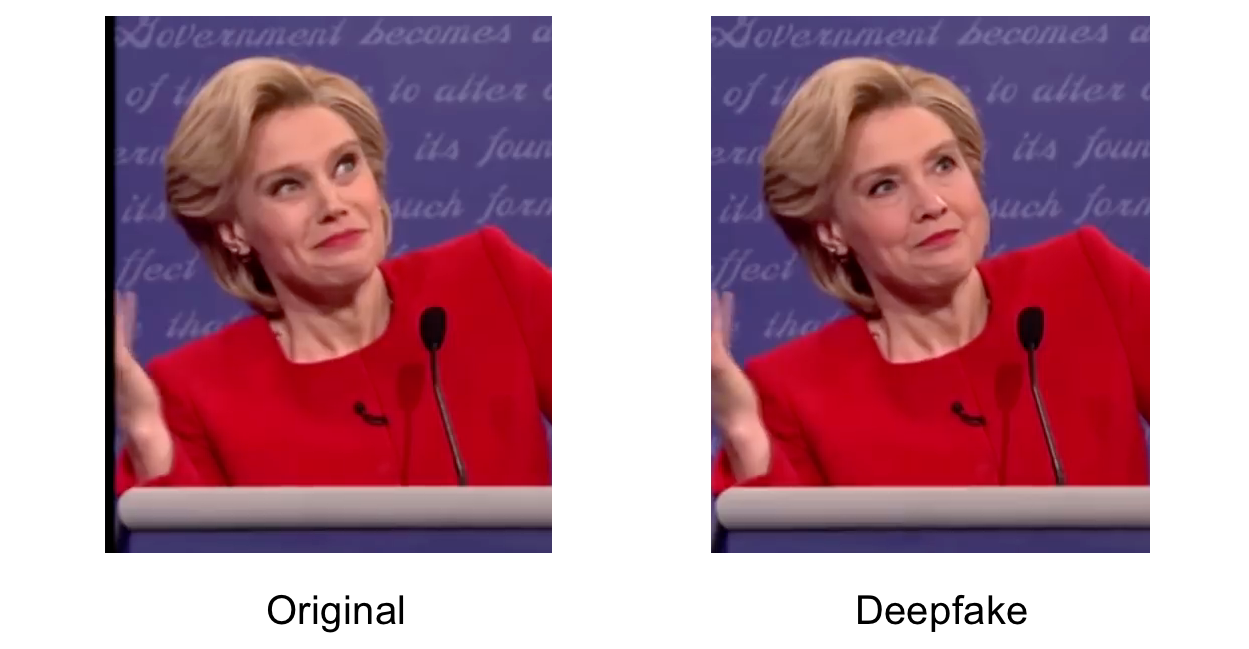
\includegraphics[width=0.9\textwidth]{img/deepfake_example.png}
        \caption{Hilary Clinton deep faked on photo}
        \label{fig:hilary-clinton-faceswap}
    \end{figure}
\end{frame}

\begin{frame}[containsverbatim]{Tackling actual problem}
    \begin{figure}
        \centering
        
\includegraphics[width=0.8\textwidth]{img/trump.png}
        \caption{Fake image of Donald Trump being arested}
    \end{figure}
\end{frame}
\section{Actual content}

\begin{frame}[containsverbatim]{FaceForensics++}
    \begin{figure}
    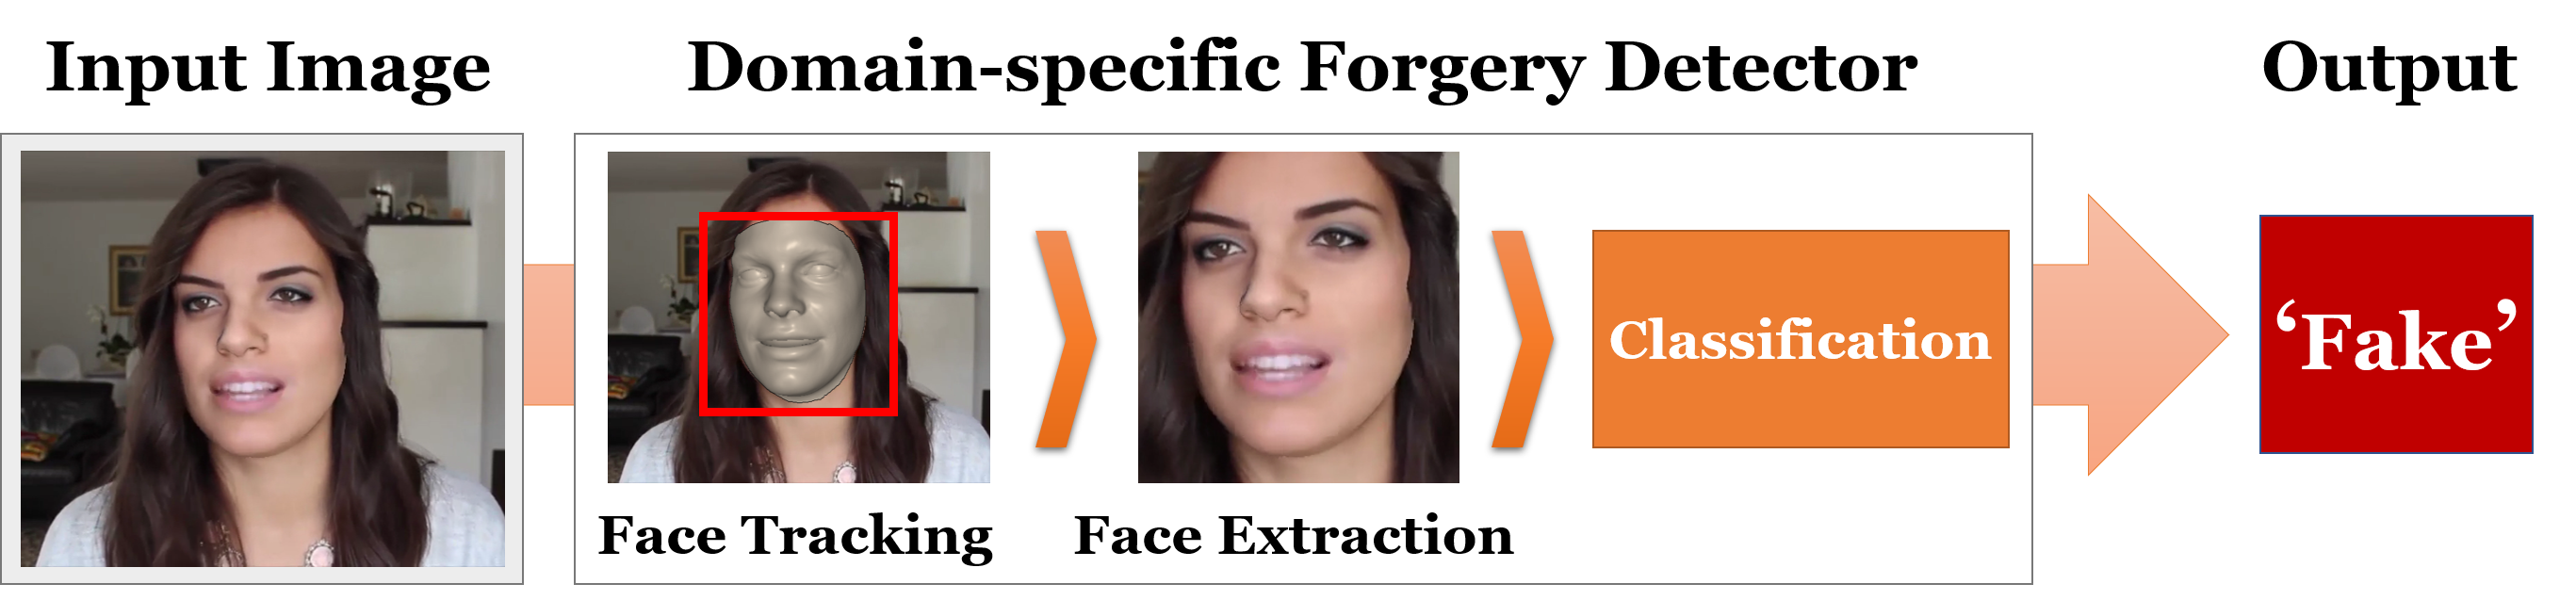
\includegraphics[width=\linewidth]{img/FF++detection_pipeline.png}
    \caption{ Visualization of FaceForensics++.
  Source: \cite{rossler2019faceforensics++}}
    \label{img:FFPileline}
    \end{figure}
\end{frame}


\begin{frame}[containsverbatim]{ManTra-Net}
    \begin{figure}
    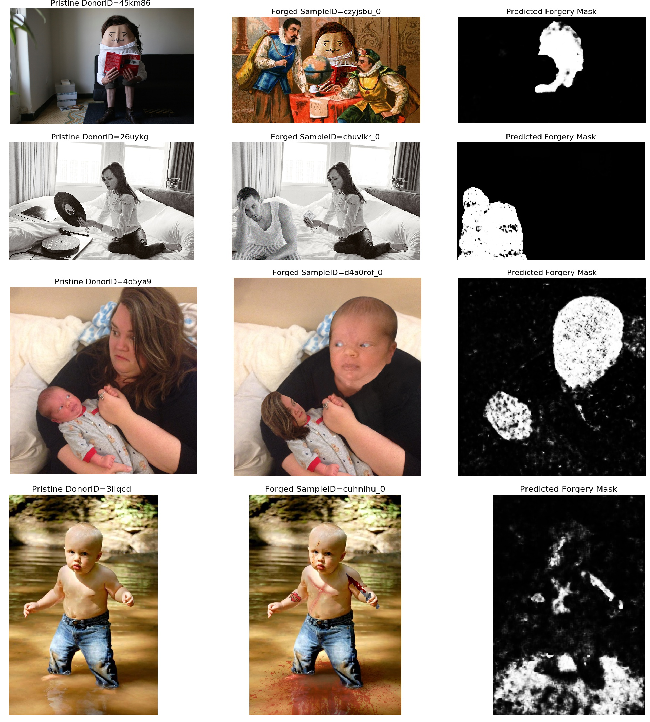
\includegraphics[width=0.5\linewidth]{img/mantra-net-example.png}
        \caption{Results of  Mantra-Net.  Source: \cite{ManTraNet}}
    \label{img:mantra-net}
    \end{figure}
\end{frame}

\begin{frame}[containsverbatim]{Conclusion}
\begin{block}{}
 Detection of ML altered images was possible at that point in time. 
\end{block}
\end{frame}

\section{Sources}

\begin{frame}[allowframebreaks]{Bibliography}

\begin{thebibliography}{99}
\bibliographystyle{ieeetr}
\bibliography{ref} 
\end{thebibliography}

\end{frame}

\end{document}

